\newpage

\section{Funcionalitats de la web}

\subsection{Calcular el total d'una compra.}


\subsection{Aplicar el descompte de client a $n$ productes de supermercat}

\begin{verbatim}
    db.Products.aggregate([
    {
    $project:
        {
            "name":1,
            "price":1,
            "discount":
            {
                $sum:[
                        "$price",
                        {
                        $multiply:["$price", -0.8]
                        }
                    ]
            }
        }
    }
    ])
\end{verbatim}

\begin{figure}[htpb!]
    \centering
    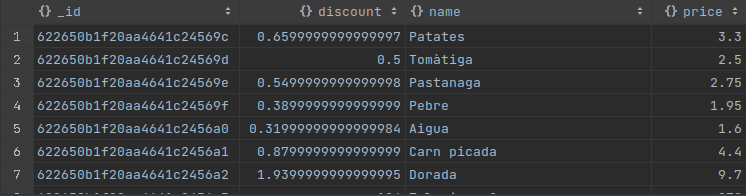
\includegraphics[width=400pt]{figures/discount.png}
\end{figure}

\subsection{Afegir un cupón}

\begin{verbatim}
    db.Users.updateOne(
        {
            username: "alopecia"
        },
        {
            $set: {
            "cupón":["Alimentació","10"]
        }
        }
    )
\end{verbatim}

\begin{figure}[htpb!]
    \centering
    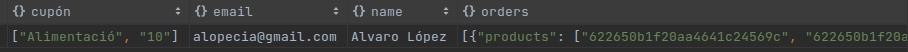
\includegraphics[width=400pt]{figures/cupon.png}
\end{figure}

\subsection{Filtrar productes per categoría}

\begin{verbatim}
    db.Products.find(
                        {
                            category:"Nom de la categoria"
                        }
                    )
\end{verbatim}

\begin{figure}[htpb!]
    \centering
    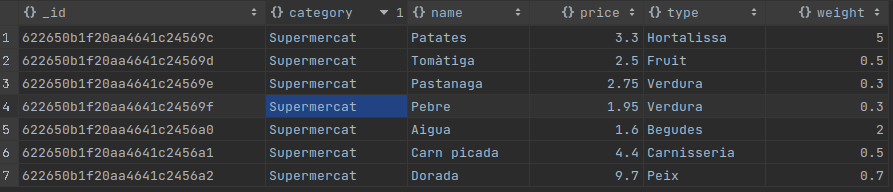
\includegraphics[width=400pt]{figures/Filtratge categories.png}
\end{figure}

\subsection{Filtrar productes per preu}

\begin{verbatim}
    db.Products.find(
                        {
                            price:{ $lt: 10}
                        }
                    )
\end{verbatim}

\begin{figure}[htpb!]
    \centering
    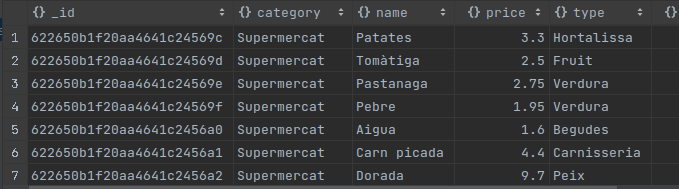
\includegraphics[width=400pt]{figures/preu.png}
\end{figure}

\subsection{Filtrar productes per tenda}

\subsection{Buscar productes}

\begin{verbatim}
    db.Products.find(
                        {
                            name:"Nom del producte"
                        }
                    )
\end{verbatim}

\begin{figure}[htpb!]
    \centering
    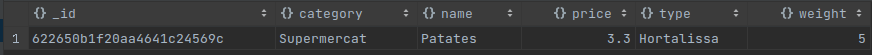
\includegraphics[width=400pt]{figures/Buscar productes.png}
\end{figure}

\subsection{Buscar productes d'una compra passada}

\begin{verbatim}
    db.Users.find(
                    {
                        username:"marieta13",
                        "orders.order_date":"2021-24-08 12:34:21"
                    },
                    {
                        _id:0,"orders.products":1
                    }
                )
\end{verbatim}

\newpage

\subsection{Un usuari es canvia el nom.}

\begin{verbatim}
    db.Users.updateOne(
                        {username:"marieta12"},
                        {$set:{"username":"marieta13"}}
                      )
\end{verbatim}

\begin{figure}[htpb!]
    \centering
    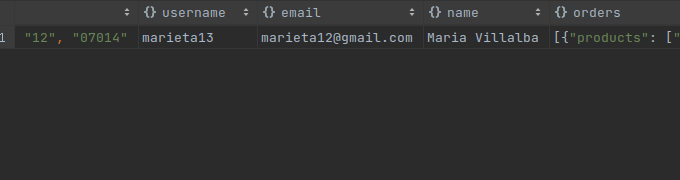
\includegraphics[width=400pt]{figures/maria.png}
\end{figure}

\subsection{Comptar quantitat de pedidos per un usuari}

\begin{verbatim}
    db.Users.aggregate([
    {
    $match: { username: "marieta13"}
    },
    {
    $project: {
               NumberOfOrders: {$size:"$orders"}
              }
    }
    ])
\end{verbatim}

\begin{figure}[htpb!]
    \centering
    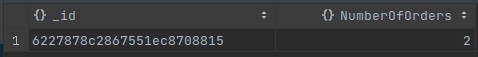
\includegraphics[width=400pt]{figures/orders.png}
\end{figure}